\documentclass[10pt,letterpaper]{article}

\usepackage{cogsci}
\usepackage{pslatex}
\usepackage{pdfsync}
\usepackage{apacite2}
\usepackage{amsmath}
\usepackage{graphicx}
\usepackage{topcapt}
\usepackage{color}

\title{A Pragmatic Account of the Processing of Negative Sentences}
\author{{\large \bf Ann E. Nordmeyer} \\ \texttt{anordmey@stanford.edu}\\ Department of Psychology \\ Stanford University \\ 
\And {\large \bf Michael C. Frank} \\ \texttt{mcfrank@stanford.edu} \\ Department of Psychology \\ Stanford University \\ }

\begin{document}
\maketitle

\begin{abstract}

Previous work suggests that negative sentences are more difficult to process than positive sentences (e.g.\ \citeNP{hclark1972}). A supportive context, however, can mitigate this effect (e.g.\ \citeNP{wason1965}).  We investigate the role of context on negation by measuring the processing cost of negation with and without a visual context (Study 1) and then systematically varying the strength of the context (Study 2).  We find that a supportive visual context has a graded effect on negation processing.  We then create a model to compute the informativeness of an utterance in context, and find that a model that considers both the surprisal of an utterance and the surprisal of seeing a referent is highly correlated with reaction times.  This suggests that a theory of pragmatic surprisal can explain the processing cost of negation.  

\textbf{Keywords:} 
Negation; sentence processing; pragmatics
\end{abstract}

\section{Introduction}

Language is a powerful tool that allows us to describe not only the state of the world as we see it, but also the world as it is not.  If I am a regular at a coffee shop and always order chai, but the shop has run out today, the barista might say ``We don't have any chai today'' when I enter.  Negative sentences are very informative when expectations are violated.

Although negation is critical for communicating many meanings, processing negation can be slow and effortful.  In sentence verification tasks, participants who are asked to evaluate the truth of a sentence describing a picture take significantly longer to evaluate negative sentences compared to positive ones \cite{hclark1972, carpenter1975, just1971, just1976}. In EEG experiments, sentences in which the final noun is semantically unexpected elicit an N400 response, and this response is found even when a negative makes the sentence logically true (e.g.\ ``A robin [is/is not] a truck'')---suggesting that negation is slow to integrate with the rest of the sentence \cite{fischler1983, ludtke2008}.  Similar results have been found in probe-recognition tasks \cite{kaup2003, kaup2006, hasson2006}.  Collectively, this work suggests that negative sentences can be quite difficult to process.
 
There is a critical difference, however, between evaluating a sentence in the lab and comprehending speech in the real world. According to Grice's Cooperative Principle \cite{grice1975}, speakers should produce utterances that are truthful, relevant, and informative.  Negative sentences presented without context violate this principle.  If the barista says ``we don't have chai today'' to a customer who always orders coffee, this utterance would be neither relevant nor informative.  In general, negations are produced when there is some expectation that the speaker wishes to reverse.  

Congruent with this Gricean account, a number of studies have shown that a supportive context mitigates the processing cost of negation.  \cite{wason1965, glenberg1999, ludtke2006, nieuwland2008, dale2011}. Some contexts are more effective than others at reducing processing demands. For example, contexts that explicitly mention a negated characteristic \cite{ludtke2006} or that present the negation within a dialogue \cite{dale2011} elicit faster reaction times, perhaps because the negation is more informative. But although these findings are congruent with the idea that pragmatic expectations are the source of negation's processing cost, they do not directly test that hypothesis.  The goal of our current work is to make such a test.

We propose that negative sentences are more informative in contexts that set up a strong expectation that is violated. If the processing cost of negation is pragmatic, then more informative negative sentences should elicit smaller reaction times. How should we quantify informativeness in context? Recent modeling work quantifies pragmatic reasoning in simple experimental contexts \cite{frank2012,goodman2013}. The assumption underlying this work is that speakers are informative---they will produce utterances that will pick out smaller subsets of the context, leaving as little ambiguity as possible for the listener.  We use this definition of informativeness to provide a quantitative interpretation of our hypothesis.

To link informativeness---as computed in a probabilistic model---to reaction time, we assume that reaction time is proportional to \emph{surprisal}. Surprisal is an information-theoretic measure of the amount of information carried by an event (in this case, an utterance in some context) based on its probability. Surprisal has been used effectively to predict reaction times from probabilistic models \cite{levy2008}; this work provides inspiration for our current model. 

We test the hypothesis that pragmatic surprisal explains the processing cost of negative sentences. Study 1 measures this processing cost, replicating previous findings that context facilitates the processing of negation.  Study 2 investigates the effect of the strength of the context by parametrically varying the base rate of a negated feature.  We compute the surprisal of sentences in these contexts, and find that a model of pragmatic informativeness predicts the relationship between context and reaction time.  These results support the idea that context affects negative sentence processing by modulating listeners' expectations. 

\section{Study 1: Context vs. No Context}

To test whether non-linguistic contextual expectations alleviate the processing cost of negative sentences, we constructed a simple sentence verification task based on \citeA{hclark1972}.  Previous studies of the relationship between context and negation have required participants to actively engage with the context, either by describing pictures \cite{wason1965} or reading sentences \cite{glenberg1999}.  Here, participants passively viewed a visual context, eliminating linguistic confounds in previous work.  

\subsection{Method}

\subsubsection{Participants}

We recruited 100 participants to participate in an online experiment through the Amazon's Mechanical Turk (mTurk) website.\footnote{Previous work has shown that mTurk is an effective tool for collecting RT data \cite{crump2013}.}  Participants ranged in age from 18-65; 63 were male and 37 female.  We restricted participation to individuals in the United States. We paid participants 30 cents to participate, which took approximately 5 minutes to complete.  

\subsubsection{Stimuli}

\begin{figure}[t]
\begin{center} 
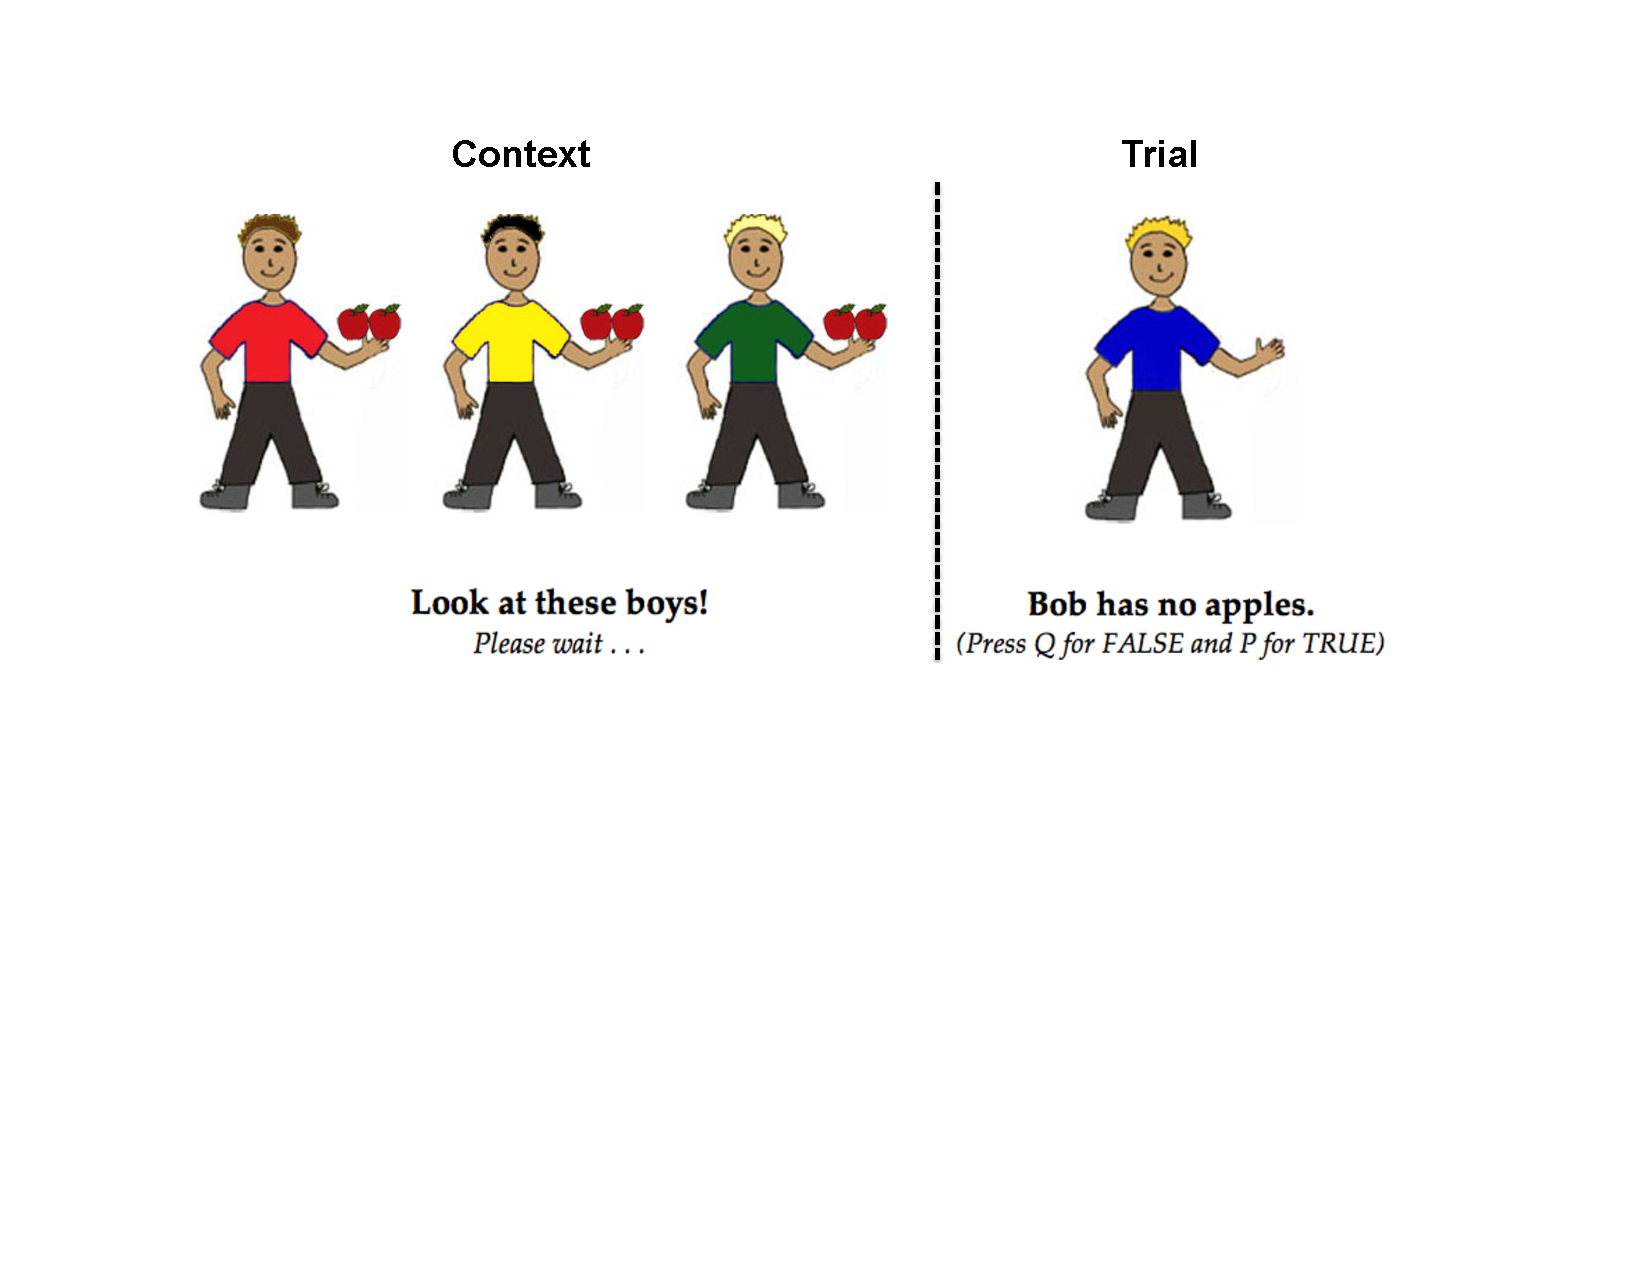
\includegraphics[width=3.25in]{figures/negatron_trialfig2.pdf}
\caption{\label{fig:trial} An example trial, consisting of two separate slides (shown sequentially): a context slide and a trial slide for a true negative trial. }
\vspace{-5mm}
\end{center} 
\end{figure}

Twenty-eight trial items were created in which a character was shown holding either two of the same common, recognizable objects (e.g.\ two apples), or holding nothing.  On each trial a sentence of the form ``[NAME] has/has no [ITEM]'' was written.  Half of the sentences were positive and half were negative, and they were paired with pictures such that half were true and half were false.  The experiment was fully crossed, with participants receiving seven true positive, seven false positive, seven true negative and seven false negative sentences in a randomized order over the course of the study.  

Participants were randomly assigned to the ``no context'' condition or the ``context'' condition.  Participants in the no context condition saw a blank screen with a fixation cross before each trial, while participants in the context condition viewed a context slide.  The context slide showed three characters, each holding the same two identical items.  The characters all differed from the trial character and from each other in hair and shirt color.  A sentence instructed participants to ``Look at these [boys/girls]!'' (Fig.\ \ref{fig:trial}).  


\subsubsection{Procedure}
Participants were first presented with an instructions screen which described the task and informed them that they could stop at any time.  Once they accepted the task, they were given eight positive sentence practice trials with feedback about incorrect responses. 

In each trial, participants saw a context (3s) and then a picture and a sentence. They were asked to read the sentence and respond as quickly and accurately as possible with a judgment of whether it was true or false when applied to the picture.  We recorded reaction times for each trial, measured as the time from when the pictures/sentence were presented to the moment when the response was made.

\subsubsection{Data Processing}
We excluded from analysis 6 participants who did not list English as their native language, 7 participants for having participated in a previous iteration of the experiment, and 4 participants for having an overall accuracy of below 80\%.  Thus, data from a total of 83 participants were analyzed.  We also excluded trials with RTs greater than 3 standard deviations from the log-transformed mean.  

\subsection{Results \& Discussion}

\begin{figure}
\begin{center} 
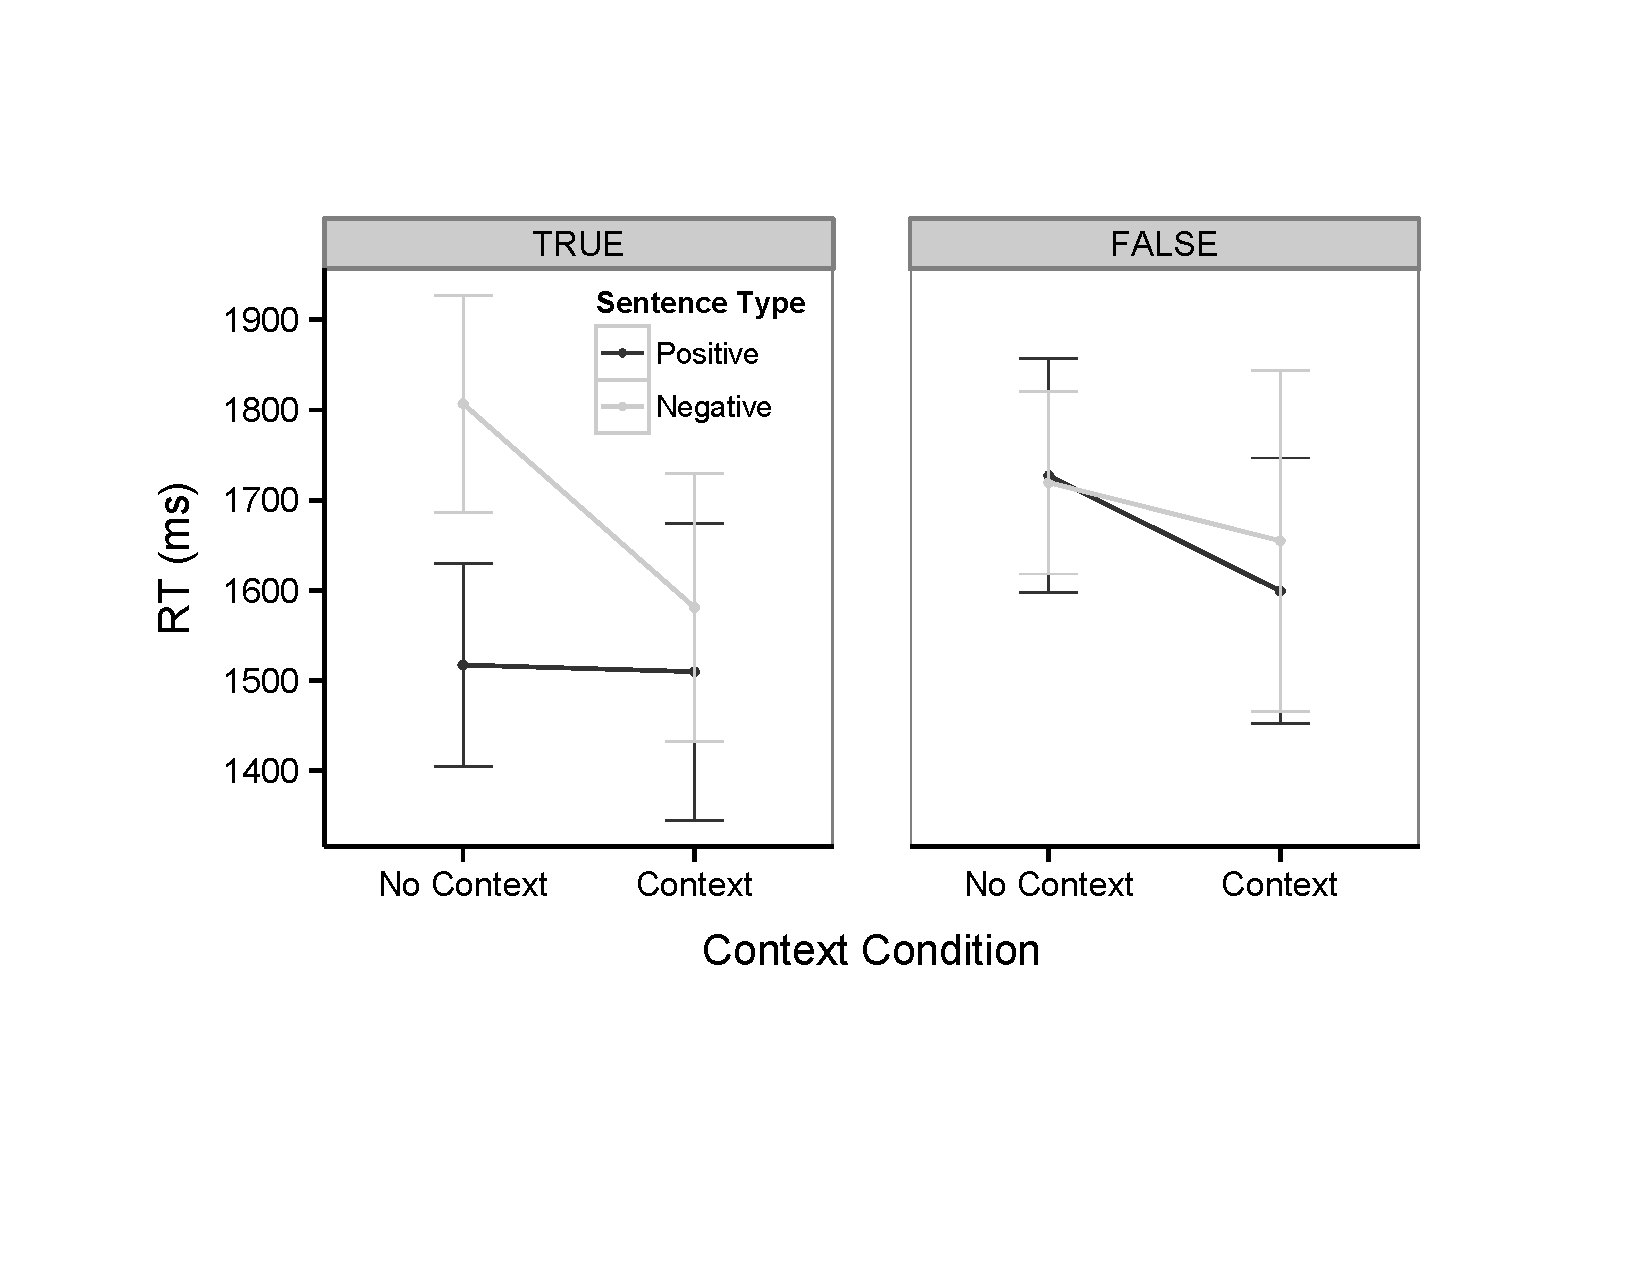
\includegraphics[width=3.25in]{figures/study1_linegraph.pdf}
\caption{\label{fig:e1line} Reaction times for each trial type across different conditions.  Responses to true sentences are shown on the left, and false sentences are shown on the right.  Negative sentences are shown in grey, and positive sentences in black.  Error bars show 95\% confidence intervals.}
\end{center} 
\end{figure}

Negative sentences were difficult to process when presented without context; in context, this effect disappeared (Fig.\ \ref{fig:e1line}).  This result is congruent with previous work on sentence verification, which has also found a main effect of negation \cite<e.g.>{hclark1972} and with work examining the role of context in negation \cite<e.g.>{wason1965, nieuwland2008, dale2011}.  

To examine the reliability of these findings, we fit a linear mixed-effects model to participants' reaction times.  We examined the interaction between sentence type, truth value, and context on reaction times.\footnote{All mixed-effects models were fit using the lme4 package in R version 2.15.3.  The model specification was as follows: \texttt{RT $\sim$ sentence~$\times$~truth~$\times$~context + (sentence~$\times$~truth~\textbar~subject) +  (sentence~$\times$~truth~\textbar~item)}.  Significance was calculated using the standard normal approximation to the $t$ distribution \cite{barr2013}.}  Results of this model show a main effect of truth value, with significant faster reaction times for true sentences compared to false sentences ($\beta= -296$, $p< .001$).\footnote{Coefficient weights are interpretable in milliseconds.}  Although there was no main effect of negation across both conditions, there was an interaction between sentence type and truth value ($\beta= 260$, $p< .001$), replicating the finding that participants respond fastest to true positive sentences but slowest to true negative sentences \cite{hclark1972}.  Critically, there was a significant 3-way interaction between context condition, sentence type, and truth value ($\beta= -227$, $p< .01$), suggesting that this interaction was primarily driven by the slow RTs for true negative sentences in the no context condition.  

To understand why context had the strongest effect on true negative sentences, consider what a true negative trial looks like in the no context condition.  These are trials in which the participant has no expectation about what the character might be holding, because no context was provided to set up such an expectation.  The participant would then see a picture of an empty-handed boy with the sentence ``Bob has no apples.''  These types of trials likely cause participants to falter because there is no reason for ``apples'' to be mentioned at all.  However, when a participant first views a context such as the one in Fig.\ \ref{fig:trial}, they can form an expectation that boys typically have apples.  Now, when participants see a boy with no apples, a sentence such as ``Bob has no apples'' makes sense.

Study 1 contributes to a body of evidence suggesting that negative sentences are more felicitous when they negate an expectation, and that such expectations can be set up by an appropriate context.  In Study 2, we examine how systematically manipulating the strength of the context might produce changes in reaction times by altering the expectations created by the context.  

\section{Study 2: Varying strength of context}

Should all contexts be equally helpful in processing negation? In Study 2, we parametrically manipulated the strength of the context.  Participants saw contexts consisting of either three (Study 2a) or four (Study 2b) characters in which some subset of the characters were holding the target item.  If the context gives participants a glimpse into the ``world'' that each trial exists in, this represents a small sample of the base rate of what the characters in this world look like.  By manipulating this base rate, we can change peoples' expectations about the trial character.  If the differences in reaction times between the no context and the context condition in Study 1 are due to the relative informativeness of the negative utterance based on the context, we should expect to see a relationship between the strength of the context and reaction time. 

\subsection{Method}

\subsubsection{Participants} 

We again recruited participants from mTurk, 200 in 2a (129 male, 71 female) and  400 in 2b (205 male, 195 female), ages 18 -- \textgreater65. We again restricted participation to individuals in the US and paid 30 cents for this 5 minute study.  

\subsubsection{Stimuli}

Study 2a used the same 28 trial items and sentence types as those used in Study 1.  A between-subjects factor determined what type of context participants saw.  Context conditions showed $\frac{0}{3}$, $\frac{1}{3}$, $\frac{2}{3}$, or $\frac{3}{3}$ of the characters holding objects.  Trial stimuli were identical to those in Study 1.  

Study 2b used 48 items.  The contexts were the same as in Study 2a, except that each context contained 4 characters and there were therefore 5 context conditions ($\frac{0}{4}$, $\frac{1}{4}$, $\frac{2}{4}$, $\frac{3}{4}$ or $\frac{4}{4}$).  

\subsubsection{Procedure}
 The procedure for Study 2a was identical to that of Study 1, with participants randomly assigned to condition.   In Study 2b, participants were given 4s (instead of 3s) to view the context before the experiment advanced.  This latency was changed to give participants more time to look at the slightly larger contexts; the procedure was otherwise identical.
 
 \subsubsection{Data Processing}
We excluded 35 participants who did not list English as their native language (9 in 2a and 16 in 2b), 24 participants for participating in a previous iteration of the experiment (3 in 2a and 21 in 2b), and 35 participants for having an overall accuracy below 80\% (11 in 2a and 24 in 2b).  Thus, we analyzed data from a total of 177 participants in Study 2a and 339 participants in Study 2b. As in Study 1, we only analyzed correct trials and excluded trials with RTs greater than 3 SDs from the log-transformed mean. 

Because we were interested in the effect of context, results from these two studies were combined and analyzed together with context condition re-coded as a continuous variable by calculating the proportion of people in each context condition who had a target item (e.g.\ the $\frac{1}{3}$ condition in Study 2a was recoded as .33). 

\subsection{Results and Discussion}

\begin{figure}[t]
\begin{center} 
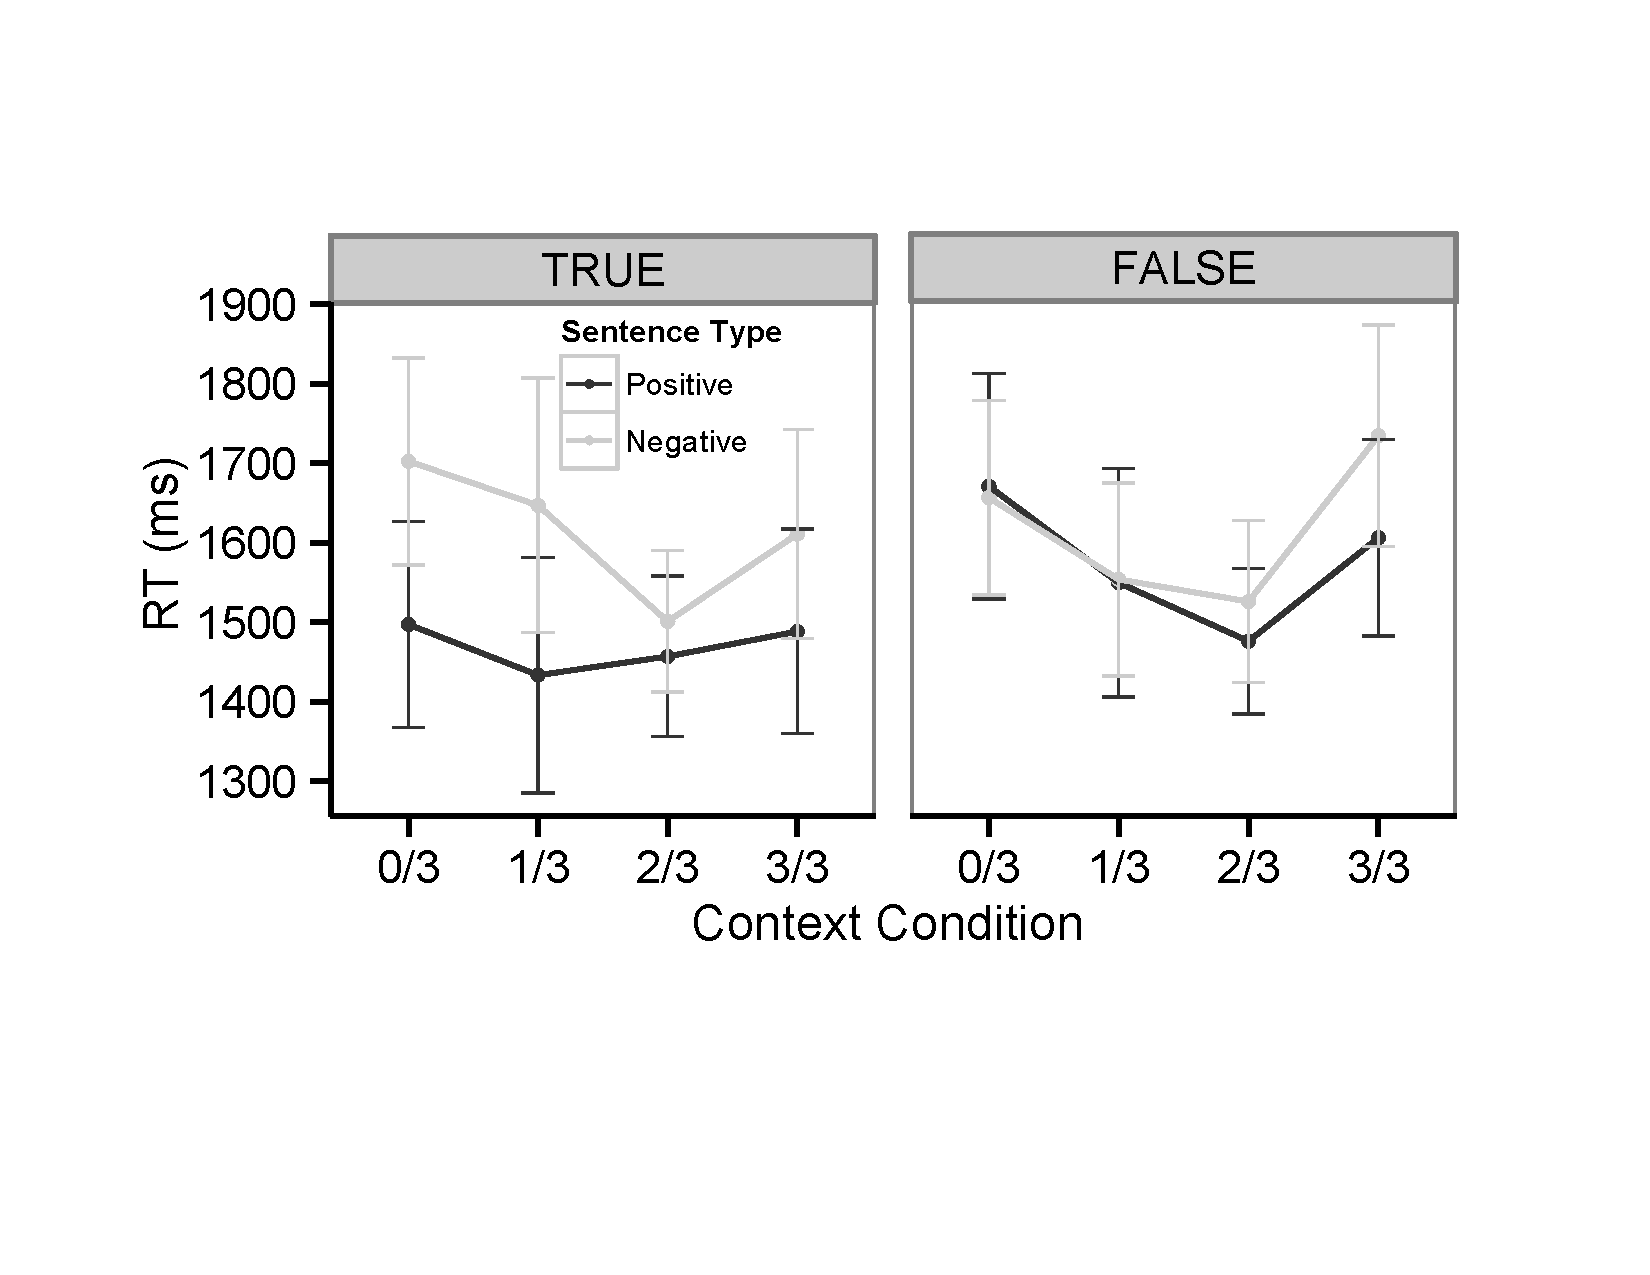
\includegraphics[width=3.25in]{figures/study2a_linegraph.pdf}
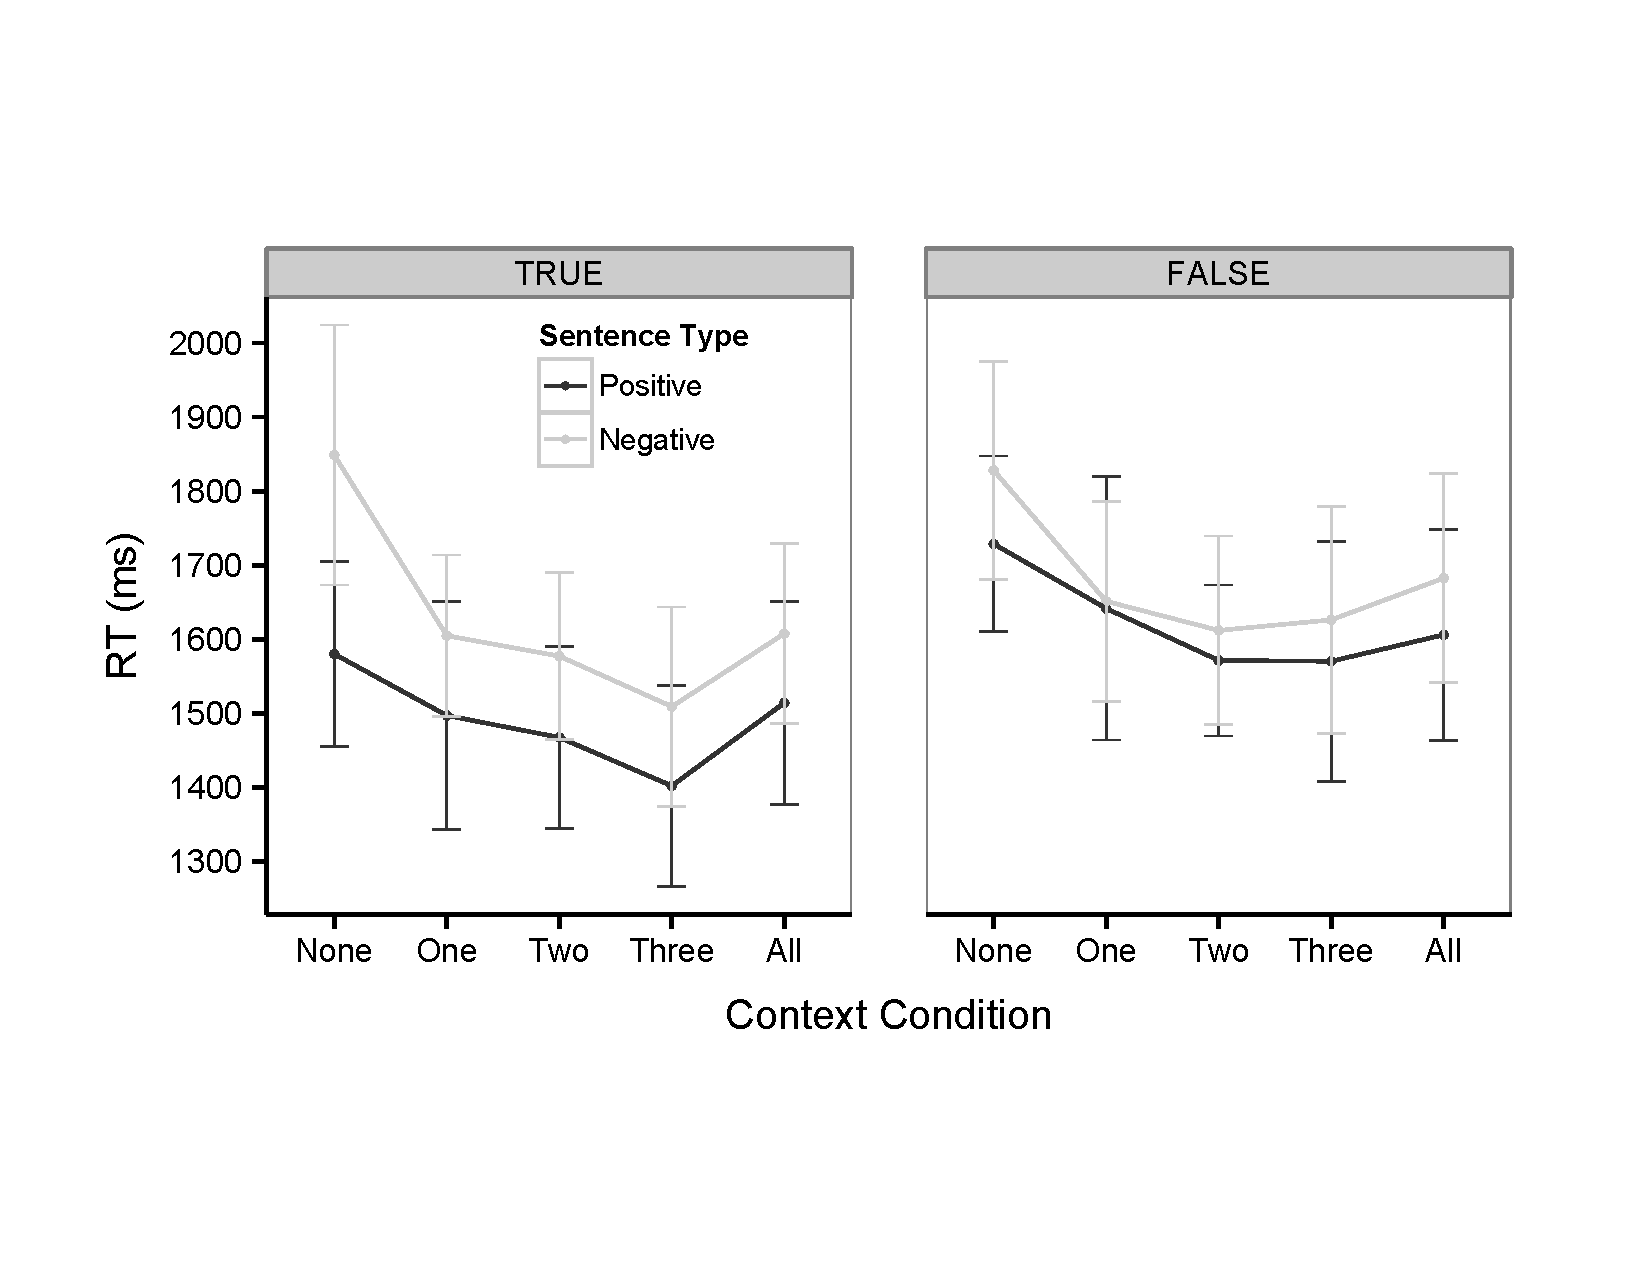
\includegraphics[width=3.25in]{figures/study2b_linegraph.pdf}
\caption{\label{fig:e2line} Reaction times for each trial type across different conditions. Responses to true sentences are shown on the left, and false sentences are shown on the right.  Negative sentences are shown in grey, and positive sentences in black.  Data for Study 2a (3-person contexts) are shown above, and data for Study 2b (4-person contexts) are shown below.  The context condition is notated by a fraction representing the number of characters in the context who held target items. Error bars show 95\% confidence intervals.  }
\end{center} 
\end{figure}

As the proportion of target items in the context increased, reaction times tended to decrease, particularly for negative and false sentences, supporting our hypothesis (Fig.\ \ref{fig:e2line}).  Unexpectedly, reaction times increased slightly when all characters in the context had target items, resulting in a U-shaped relationship between context and RT.  

We fit a linear mixed-effects model to reaction times in response to sentences.  We examined the interaction between sentence type, truth value, and context on reaction times.\footnote{The model specification was as follows: \texttt{RT $\sim$ sentence~$\times$~truth~$\times$~context + (sentence~$\times$~truth~\textbar~subject) +  (sentence~$\times$~truth~\textbar~item)}.}  As in Study 1, we found a significant effect of truth value, with significantly faster reaction times for true sentences compared to false sentences ($\beta= -154$, $p< .001$).  Although there was not a significant main effect of negation, there was a significant interaction between sentence type and truth value, such that the difference between true positive and true negative was greater than the difference between the two types of false sentences ($\beta= 159$, $p< .001$).  There was also a linear effect of context, such that as the proportion of people with the target item in the context increased, reaction times decreased ($\beta= -197$, $p< .001$).  As before, there was a significant 3-way interaction between context, sentence type, and truth value, such that the linear effect of context was most striking in true negative sentences ($\beta= -141$, $p< .001$).

Responses in the $\frac{3}{3}$ and $\frac{4}{4}$ conditions suggest that the relationship between context and RT is not linear (Fig.\ \ref{fig:e2line}).  We added a quadratic term to our model to test for this nonlinear effect of context ($\beta= 610 $, $p< .001$).  The quadratic model fit our data significantly better in a likelihood comparison test ($\chi^{2}(1) =80.59$, $p<.001$).  

Quantitative manipulation of the strength of the context resulted in systematic changes in the processing cost of negation, particularly for true negative sentences.  This finding is consistent with our initial hypothesis: As the proportion of people in the context with the target item increases, describing the trial picture as \emph{not} having that target item becomes more informative.  That is, the more people in the context who have apples, the more we expect a person with nothing to be described as ``a boy with no apples.'' 


\section{Model}

Studies 1 and 2 show that a simple visual context can facilitate the processing of negation, with contexts that set up a strong expectation leading to faster RTs for negative sentences.  We hypothesized that this effect is driven by the expectation that speakers are informative \cite{grice1975,frank2012}: If everyone in a context has a specific feature, and the target character is lacking that feature, it is highly informative to describe the target character in terms of the negation of the expected feature. In this section, we formalize this prediction. Due to the Gricean nature of this prediction, we focus here on predicting responses to true sentences.   

We modeled the behavior of participants in our experiments (following \citeNP{levy2008}) by assuming that reaction time is proportional to the surprisal of the utterance $w$, given the context $C$ and the speaker's intended referent $r_S$:

\begin{equation}\label{eq:surprise}
RT \sim -\log(P(w| r_s, C)).
\end{equation}

\noindent We then define the probability of the utterance as proportional to its utility (following \citeNP{frank2012}):

\begin{equation}\label{eq:pw1}
P(w | r_s, C) \propto  e^{U(w;r_s,C)},
\end{equation} 

\noindent This utility is defined as the informativeness of $w$ minus its cost $D(w)$:

\begin{equation}\label{eq:utility}
U(w;r_s,C) = I(w;r_s, C) - D(w).
\end{equation}

\noindent Informativeness in context is calculated as the number of bits of information conveyed by the word. We assume that $w$ has a uniform probability distribution over its extension in context (e.g.\ ``boy with apples'' applies to any boy who has apples, leading to a probability of $1/|w|$ of picking out each individual boy with apples) :

\begin{equation}\label{eq:info}
I(w;r_s, C) = -(-\log(|w|^{-1})).
\end{equation}

\noindent The cost term $D(w)$ can then be defined in any number of ways; in this model we define it as the number of words in the utterance multiplied by a cost-per-word parameter.  Note that in our experiment, the negative sentences always have exactly one word more than the positive sentences. 

We created a sparse vocabulary which represented possible words to describe the characters.  This included the target utterance (e.g.\ ``apples'' and ``no apples''), as well as words that were uniformly true or false of all characters. Combining Equations \ref{eq:pw1}--\ref{eq:info}, and normalizing Eq.\ \ref{eq:pw1} over all possible words in the vocabulary $V$, we have:

\begin{equation}\label{eq:pw2}
P(w | r_s, C) = \frac{ e^{\log(|w|^{-1}) - D(w)}} {\sum_{w' \in V}{e^{\log(|w'|^{-1}) - D(w')}}}.
\end{equation}

\noindent Combining Eq. \ref{eq:surprise} with Eq. \ref{eq:pw2}, this model predicts that as the number of e.g.\ boys with apples in the context increases, the informativeness of the negative sentence ``Bob has no apples'' increases, because it selects an increasingly smaller subset of the context. Highly informative sentences will have high probability, hence lower surprisal and faster RTs. 

We fit this model to data from Study 2a, with cost = 3 (Table 1).  When the model was fit to the combined data from Studies 2a and 2b, the cost-per-word parameter remained the same (Fig.\ \ref{fig:model1_sims}).  This model accounted for a substantial amount of variance in participant reaction times from Study 2 ($r=.76$, $p<.001$).  Nevertheless, the model fails to capture the U-shaped relationship seen in Study 2; specifically, it underestimates the surprisal of $\frac{0}{3}$ and $\frac{0}{4}$ contexts for positive sentences, and $\frac{3}{3}$ and $\frac{4}{4}$ contexts for negative sentences.

In these trials, participants may have found the target picture surprising regardless of the sentence that they read. For example, in $\frac{0}{3}$ and $\frac{0}{4}$ contexts followed by a true positive trial, participants saw several boys with nothing, and then saw a boy holding something.  To account for reaction time related to seeing the target picture, we included the surprisal of the referent $r_S$ as well as the surprisal of the utterance $w$ given the referent. We estimated the probability of seeing the referent via the count of the target property in the context, smoothed with a parameter $\lambda$:

\begin{equation}\label{eq:pp}
P(r_S | C) =  \frac{\# Matching People  + \lambda}{\# Total People + 2\lambda}
\end{equation}

We then added $-\log(p(r|C))$ (Eq.\ \ref{eq:pp}) to $-\log(p(w|r_s,C))$ (Eq.\ \ref{eq:pw2}), resulting in:

\begin{equation}\label{eq:total}
RT \sim - \log(P(w|r_s, C)) - \beta \log(P(r_S|C)).
\end{equation}

\begin{table}[t]
\caption{\label{tab:modelcorrs} Model parameters and correlations between model predictions and reaction times.  Parameters are either fit to Study 2a only or to both 2a and 2b combined as indicated.}
\begin{center}
\small\addtolength{\tabcolsep}{-2pt}
\begin{tabular}{ r r  r  r  r  r} 
\hline
  \bf{Model} & \bf{Data} & \bf{cost} & \bf{$\lambda$} & \bf{$\beta$} & \bf{$r$}  \\ \hline        
 Utterance Surprisal  &  Study 2a  & 3 & -- & -- & .84\\     
  (Model 1)& Study 2b (2a params) & 3  & -- & -- & .71\\
  & Both (2a parameters) &  3 & -- & -- & .76 \\
  & Both & 3 &  --  &  -- & .76 \\ \hline
Total Surprisal & Study 2a & .5 & .1 & .3 & .95\\     
  (Model 2) & Study 2b (2a params) & .5  & .1 & .3 & .86\\
  & Both (2a parameters) &  .5 & .1 & .3 & .89\\
  & Both & .4 &   .2 &  .4 & .90\\ 
\hline
\end{tabular}
\end{center}
\end{table}

\noindent Note that this formulation is quite similar to a model which accounts for the prior probability of the referent $p(r_S)$; the only difference is our use of a weight $\beta$ to adjust the different effects of these two probabilities.  

Consider the example in Fig.\ 1, in which you see three boys with apples and then a boy with no apples.  The sentence ``Bob has no apples'' is highly probable---and thus low surprisal---in this context, because it uniquely identifies the target character (Eq.\ \ref{eq:pw2}).  In the current model, however, we must also calculate the surprisal of seeing the target character (i.e. the referent).  In this example, the referent surprisal is high, because the probability of seeing a boy with no apples in this context is low (Eq. \ \ref{eq:pp}).  

We again fit this model to data from Study 2a and compared model predictions to data from Study 2b as well as the combined data from 2a and 2b (Table 1).  Using the parameters fit to Study 2a, the model accounted for a substantial amount of variance in participant reaction times from Study 2 ($r=.89$, $p<.001)$.  We also fit the model to the combined data from Study 2, which resulted in similar parameter values (Table 1), and continued to account for a substantial amount of the variance in RTs ($r=.90$, $p<.001$; Fig.\ \ref{fig:model1_sims}).   

\begin{figure}[t]
\begin{center} 
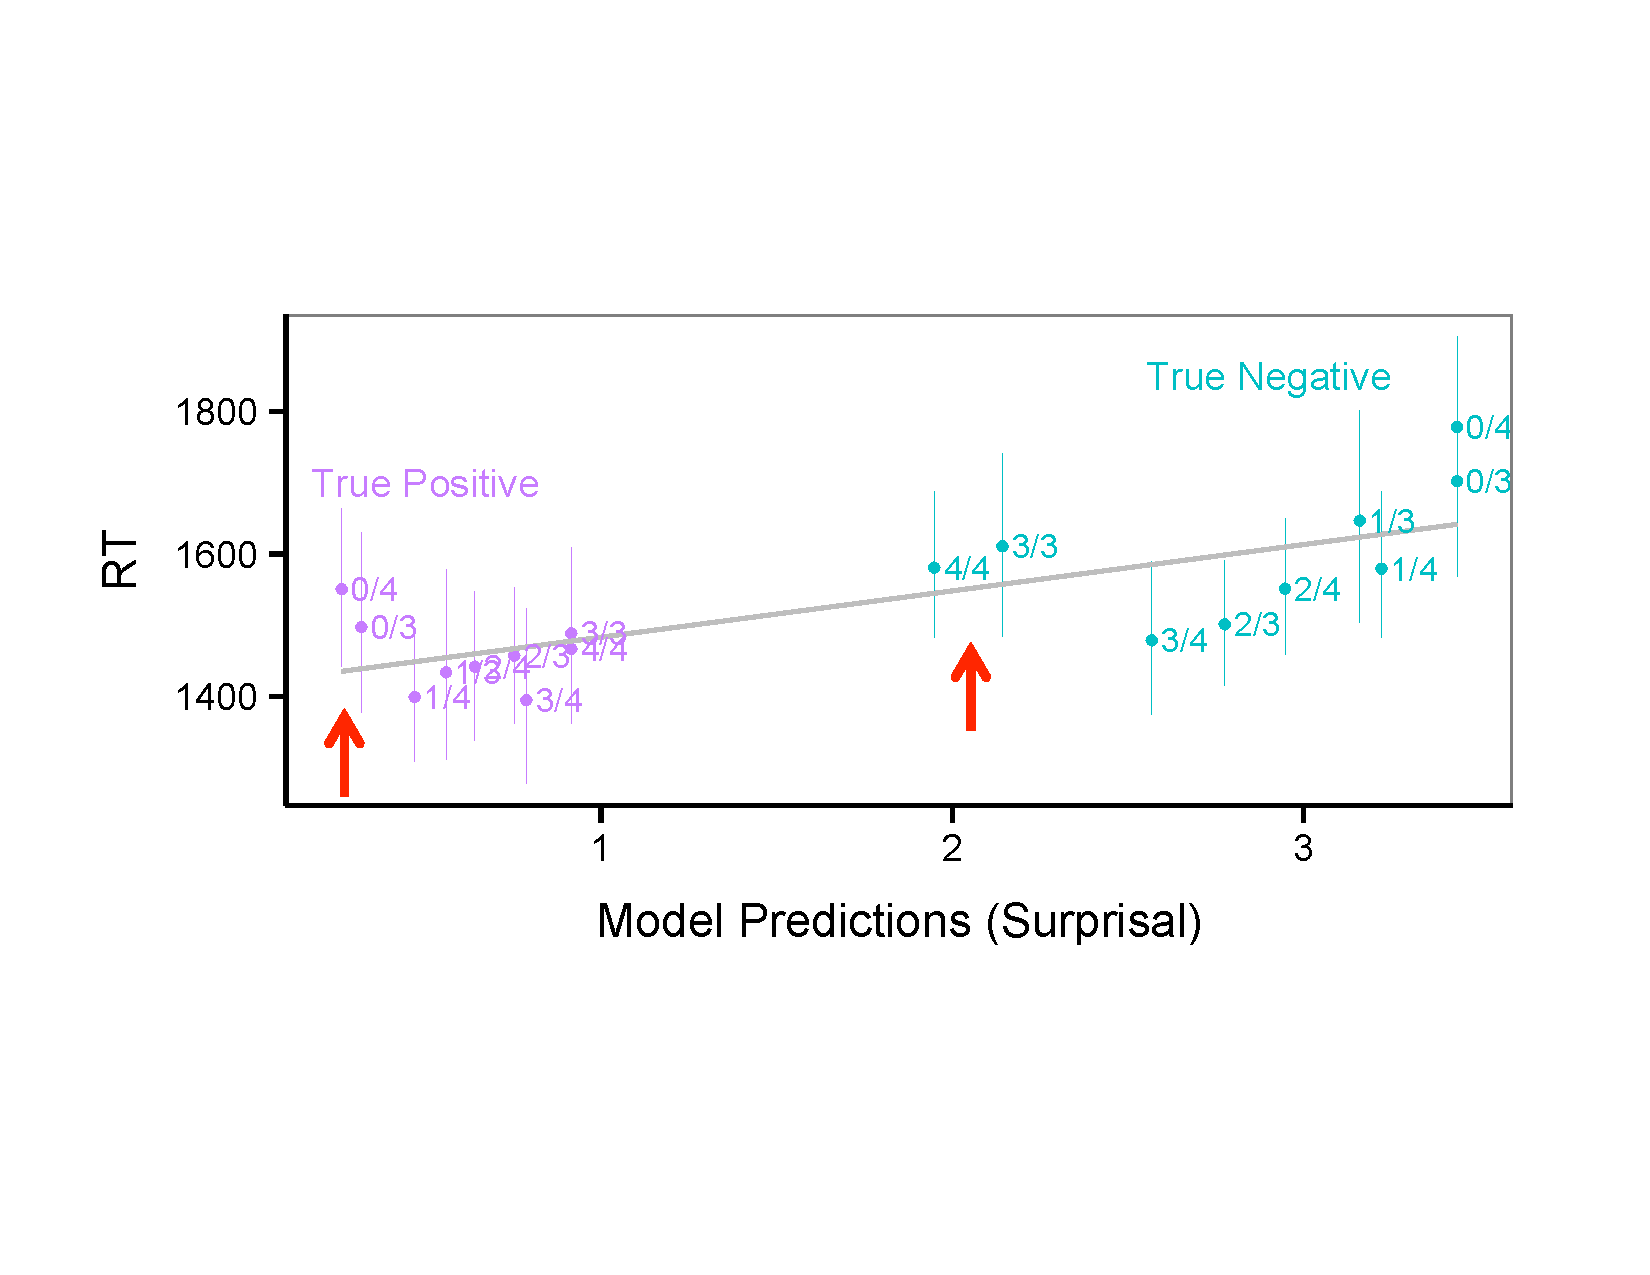
\includegraphics[width=3.25in]{figures/model1_comparison.pdf}
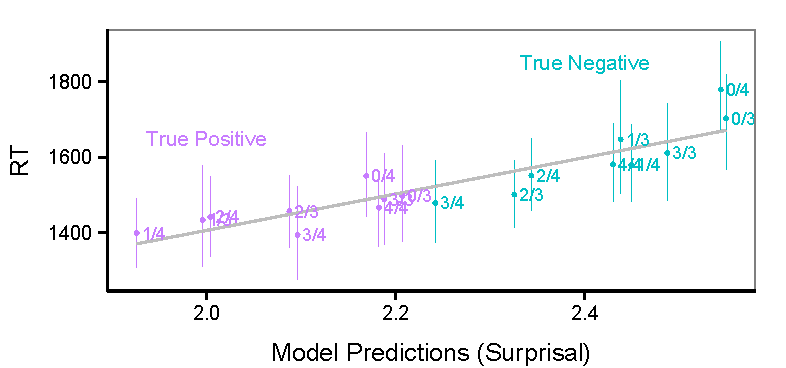
\includegraphics[width=3.25in]{figures/model2_comparison.pdf}
\caption{\label{fig:model1_sims} Best-fitting model predictions for a model of utterance surprisal (above) and a model of total surprisal, Eq.\ \ref{eq:total} (below).  Positive sentences are represented in purple and negative sentences in blue.  Context conditions are identified as fractions, written next to the relevant data point.  Arrows indicate data points that are not well captured by our initial model of utterance surprisal.}
\end{center} 
\end{figure}





\section{General Discussion}

What makes negation so hard? It takes longer to evaluate negative sentences than positive sentences when presented without context, but these effects are mitigated in context. We suggested a Gricean account: the processing cost of negation is related to the degree to which it violates expectations about communication in context. In our studies, by changing the proportion of people in the context who held a target item, we systematically manipulated participants' contextual expectations.  We found a parametric relationship between the strength of the context and reaction times, and this relationship was well fit by a model of the surprisal of a sentence and its referent given the context.

Previous work on sentence processing has suggested that processing negation is fundamentally difficult, perhaps due to the processing cost of negating a proposition (e.g.\ \citeNP{hclark1972}) or the cost of suppressing an affirmative representation (e.g.\ \citeNP{kaup2003}).  Our work here suggests that the difficulty of negation may not be unique to negation at all; instead, general pragmatic mechanisms could be driving this effect.  Due to the specific pragmatics of negation, negative sentences presented without context are uninformative and are thus unlikely to be produced, leading to increased surprisal and slower processing times.  In conversation, however, negative sentences are often produced when some expectation has been violated, decreasing surprisal and processing time.  

Although our specific focus was to understand the processing of negative sentences, this work can be extended to quantify the effect that context has on sentence processing more generally.  Debates about the effects of pragmatics on linguistic processing exist in other domains (e.g.\ the processing of scalar implicatures, \citeNP{huang2009, huang2011, grodner2010}).  Formal models of pragmatics can shed light more generally on the role that context plays in linguistic processing. 

\section{Acknowledgments}
This material is based upon work supported by the National Science Foundation Graduate Research Fellowship. Any opinion, findings, and conclusions or recommendations expressed in this material are those of the authors and do not necessarily reflect the views of the National Science Foundation.


\bibliographystyle{apacite}

\setlength{\bibleftmargin}{.125in}
\setlength{\bibindent}{-\bibleftmargin}

\bibliography{bibLibrary}

\end{document}

